\documentclass{article}

\usepackage[letterpaper, portrait, margin=1.5in]{geometry}

\usepackage{fancyhdr}
\usepackage{ragged2e}
\usepackage{graphicx}
\usepackage{caption}
\usepackage{amsmath}
\usepackage{rotating}

\usepackage{listings}
\usepackage{color}

\definecolor{dkgreen}{rgb}{0,0.6,0}
\definecolor{gray}{rgb}{0.5,0.5,0.5}
\definecolor{mauve}{rgb}{0.58,0,0.82}

\lstset{frame=tb,
  language=Java,
  aboveskip=3mm,
  belowskip=3mm,
  showstringspaces=false,
  columns=flexible,
  basicstyle={\small\ttfamily},
  numbers=none,
  numberstyle=\tiny\color{gray},
  keywordstyle=\color{blue},
  commentstyle=\color{dkgreen},
  stringstyle=\color{mauve},
  breaklines=true,
  breakatwhitespace=true,
  tabsize=4
}

\setcounter{secnumdepth}{1}

\usepackage{chngcntr}
\counterwithin{figure}{section}

\renewcommand*{\thepage}{C\arabic{page}}

\pagestyle{fancy}
\lhead{ACME Robotics}
\chead{\#8367}
\rhead{\ifcontents Contents \else Week \thesection \fi}

\newif\ifcontents
\contentstrue

\makeatletter
\renewcommand{\@seccntformat}[1]{}
\makeatother
\begin{document}
\subsection{Lift String}
%! Change the strength of the lift string
After most of the robot was completed Kelly and Aidan ran a few practice matches to make sure that everything was working properly. One thing that kept happening was the pull down string on the lift kept breaking right in the middle. This showed that the string evidently was not strong enough. The string had a 200 lb rating but evidently the impulse of the robot when going up or down was much higher than this. Kelly decided that the team should order some higher rated string to ensure that this wouldn't happen again. The team ordered a 900 lb rated string from amazon that was 3 mm thick. The team didn't know if the change in thickness from 1 mm  to 3 mm was going to cause problems so Aidan used some left over rev slides string, that was also 3 mm thick with unknown rating, to test for adverse effects because of the change in thickness. Because of the thickness of the string more slack developed when the lift raised which caused the problem of the string jumping off the spool a few times. Aidan fixed this by wrapping extra coils around the spool for the pull up run which made it so less string was released per rotation for the pull down than the pull up which fixed the problem. When the new string arrived the team now knew how to use it without problem.

\begin{figure}
    \centering
    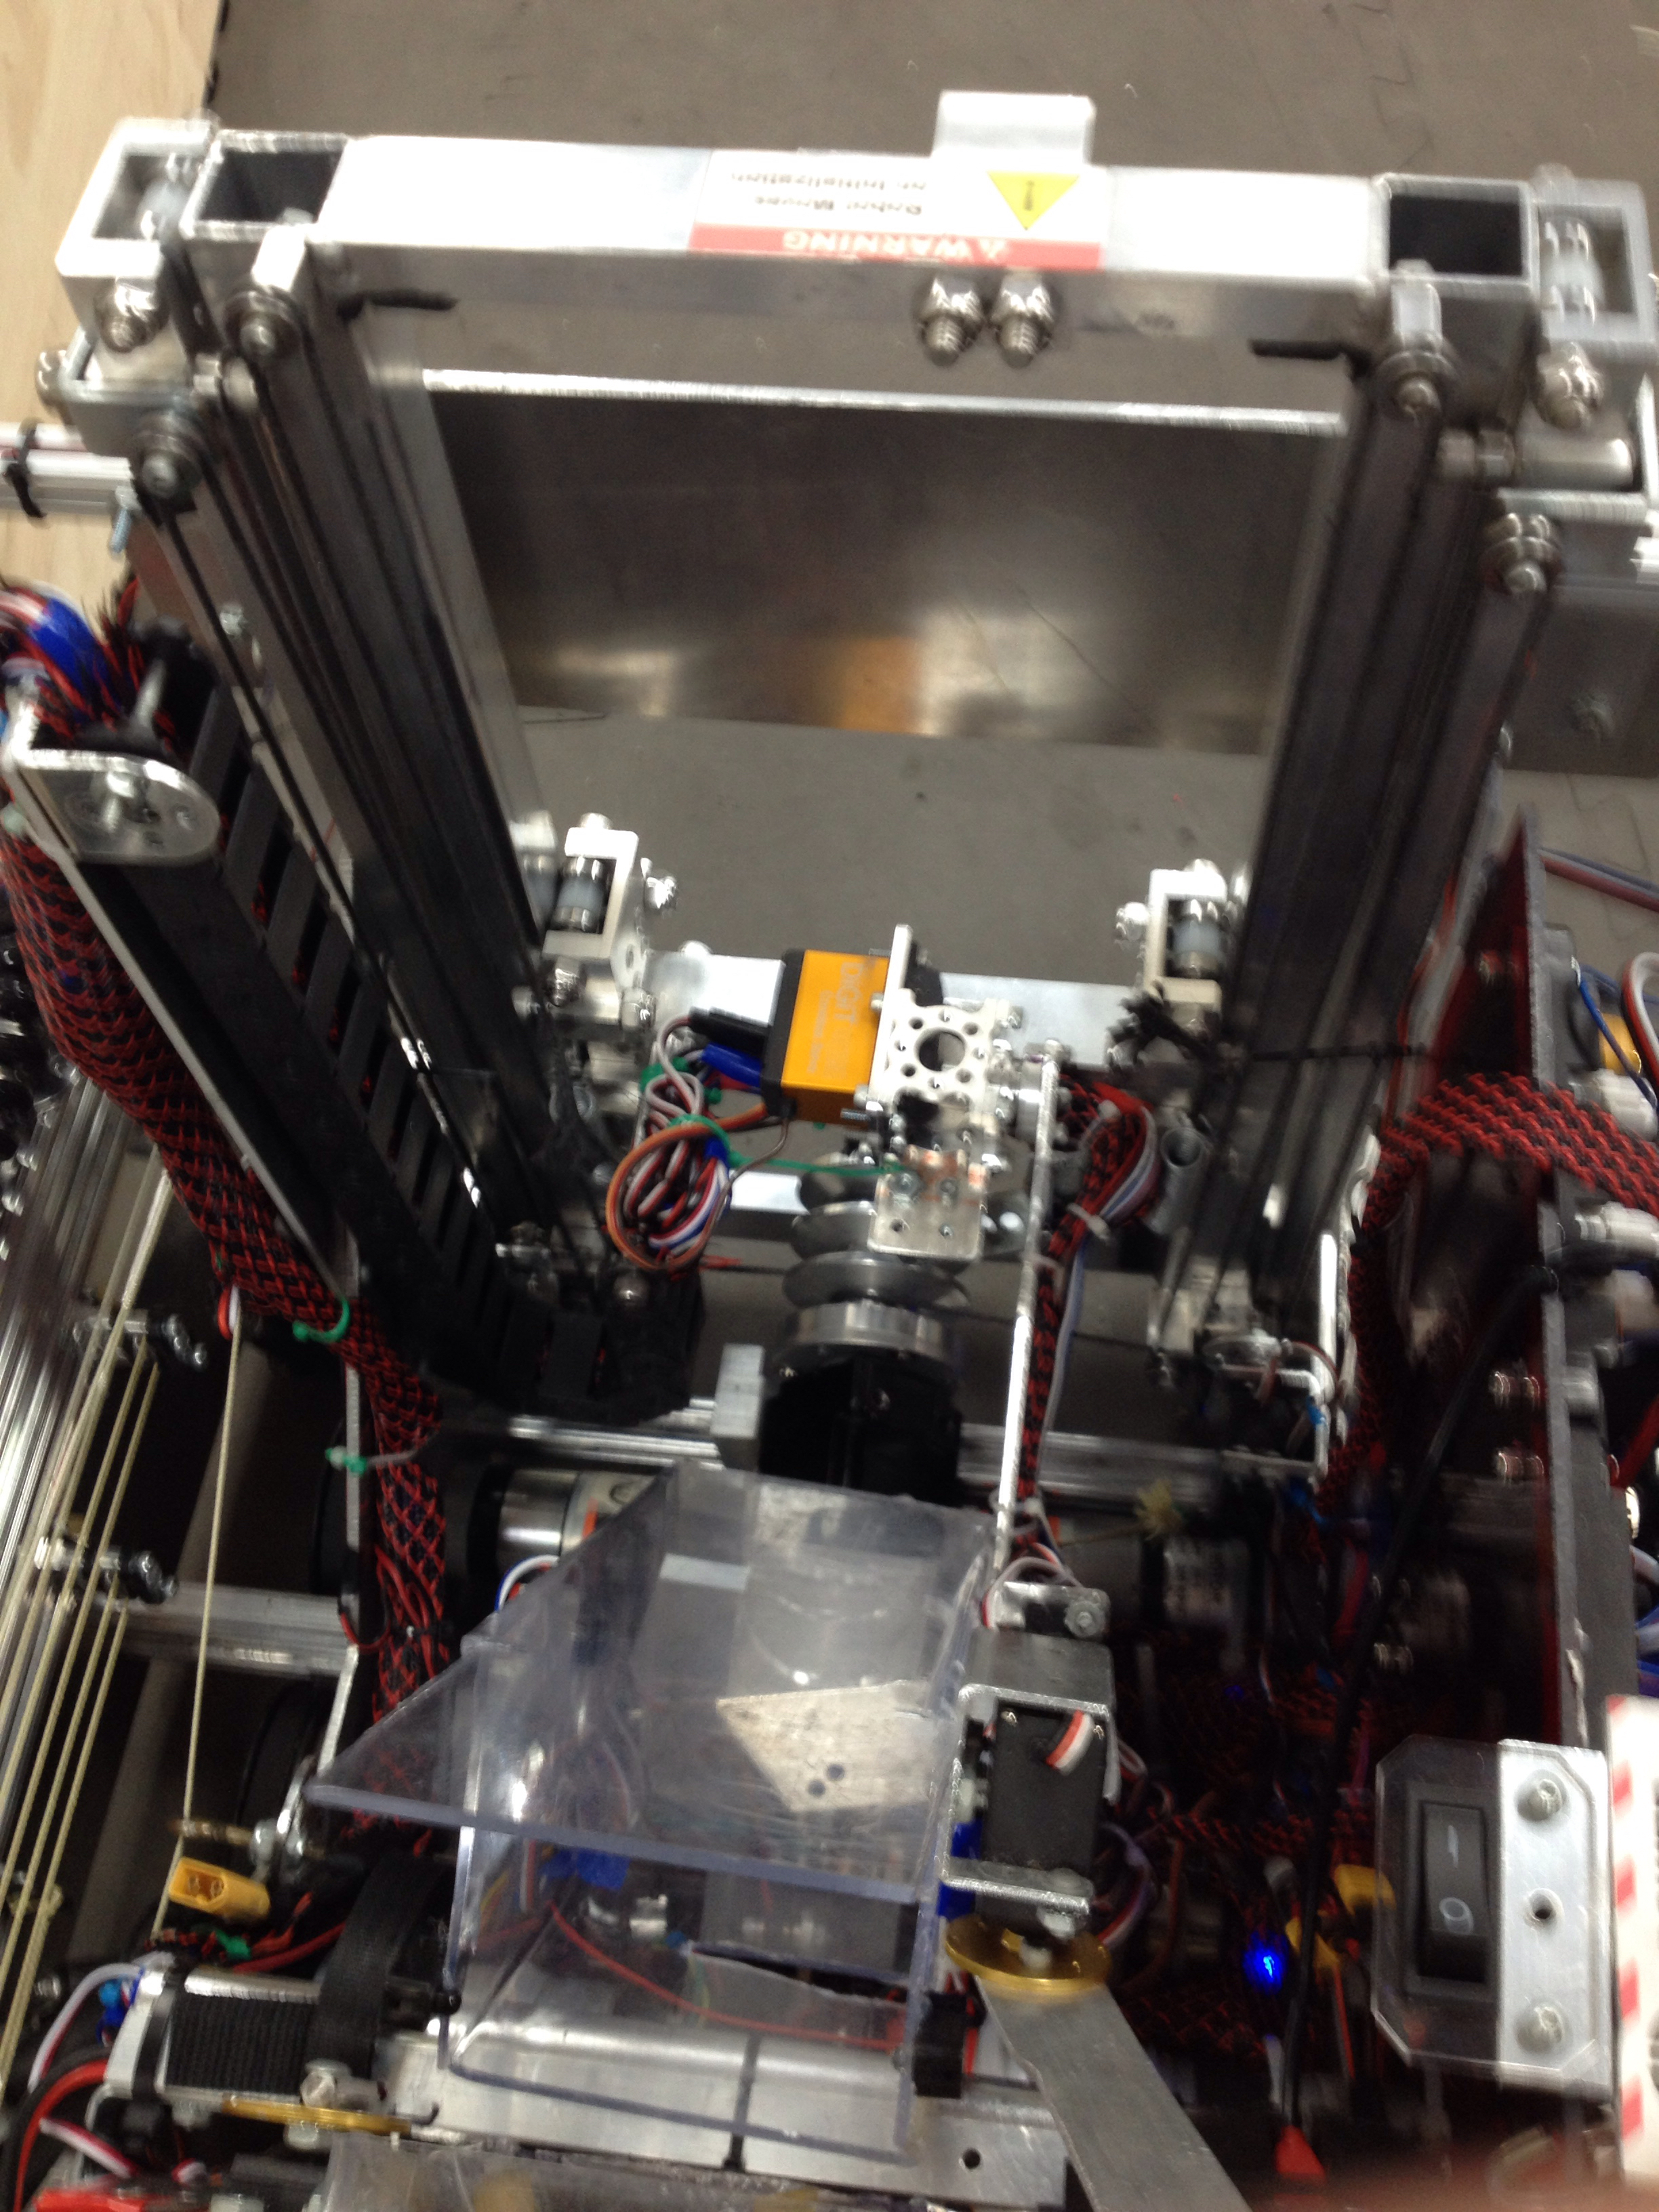
\includegraphics[width=.6 \textwidth]{22_01-28/images/thing1.jpg}
    \caption{Marker Placer}
    \label{fig:markerplacer}
\end{figure}

\end{document}